\documentclass{xnuthesis}
%=======导言区
%======================文献加载格式
\usepackage[backend=biber,style=gb7714-2015, gbalign=gb7714-2015,gbnamefmt =lowercase]{biblatex}
\addbibresource{refs.bib}
%=========信息录入
\xnxyInfo{
 session={2024届},
 id ={20201405xxxx}, 
 displaytitle={毕业论文(设计)},
 title={基于\LaTeX 的两月半研究 \\ ---以xxx为例}, 
 author={xxx},
 department={数学与信息科学学院},
 major={计算机专业}, 
 supervisor={指导老师}, 
 assocsupervisor={副导师}, 
 date={2024年5月}
}

\usepackage{enumitem} %item设置
\usepackage[hidelinks]{hyperref}
\hypersetup{
    colorlinks=true, % 启用颜色链接
    linkcolor=black,   % 内部链接颜色
    citecolor=green, % 引用链接颜色
    filecolor=magenta, % 文件链接颜色
    urlcolor=red        % 外部 URL 链接颜色
}
\usepackage{graphicx}
\graphicspath{{figures/}}
\DeclareGraphicsExtensions{.pdf,.eps,.png,.jpg,.jpeg}
\usepackage{ntheorem}

\let \slantint \int
\usepackage{cmupint}%直立体
\usepackage{pifont}%雪花星符号
\usepackage{booktabs} %三线表

\usepackage{subcaption}
\usepackage{amssymb}
\usepackage{xcolor}
\NewDocumentCommand{\emphasize}{m}{{\color{blue}\textbf{#1}}}
\usepackage[linesnumbered,ruled,vlined]{algorithm2e}
\usepackage{listings}
\RenewDocumentCommand{\lstlistingname}{}{代码}
\lstdefinestyle{Matlab}{
language={Matlab},
basicstyle=\zihao{5}\ttfamily,
columns=flexible,
frame=single, framerule=1pt,
backgroundcolor=\color{white},
keywordstyle=\color{blue},
commentstyle=\color{green!50!black}, % 移除 \itshape
stringstyle=\color{blue},
breaklines=true, % 允许自动换行
showspaces=false, % 不显示空格
showstringspaces=false,% string不显示空格
numbers=left, % 在左侧显示行号
numberstyle=\zihao{5}, % 行号的字体大小
numbersep=5pt, % 行号与代码的距离
xleftmargin=3em, xrightmargin=3em,
captionpos=b,% 题注在下
}
\lstdefinestyle{LaTex}{
language=[LaTeX]TeX,
basicstyle=\zihao{5}\sffamily,
columns=flexible,
frame=single, framerule=1pt,
backgroundcolor=\color{white},
keywordstyle=\color{blue},
commentstyle=\color{green!75!black}, % 移除 \itshape
stringstyle=\color{blue},
breaklines=true, % 允许自动换行
showspaces=false, % 不显示空格
showstringspaces=false,% string不显示空格
xleftmargin=3em, xrightmargin=3em,
captionpos=b,% 题注在下
}


%=========绘图包
\usepackage{tikz}
\usetikzlibrary{arrows.meta}
\usepackage[siunitx]{circuitikz}%电路图
\usepackage{fancybox}
\usetikzlibrary{calc}

%======某些地方需要伪粗体
\usepackage{xfakebold}
\usepackage{xeCJKfntef}%下划线兼容问题

\setcounter{tocdepth}{2} % 设置目录深度为2 %配置文件,自由加载宏包与论文的信息
 
\begin{document}
%=======封面
%-------------------自己写的封面非官方
\newcommand{\ulineshort}[1]{\underline{\makebox[9em][c]{#1}}}
\newcommand{\ulinelong}[1]{\underline{\makebox[22em][c]{\zihao{3} \kaishu #1}}}

%华文中宋与宋体相差不大,所以用宋体加伪粗体代替了
\newcommand{\zhongsongbf}[1]{\zihao{-3}  \songti \setBold[0.4] #1 \unsetBold} 
\newcommand{\displaytitlefont}[1]{\zihao{-0} \songti  \setBold[0.4] #1 \unsetBold }

%=========封面
\begin{titlepage}
\begin{tikzpicture}[remember picture, overlay]
\coordinate (SessionIDinfo) at (\textwidth,0);
%---------每个部分以页面中心为相对位置
\coordinate (Topic) at  (current page.center);
\coordinate (BasicInfo) at ($(current page.center)!0.5!(current page.south)$);
\coordinate (Dissertname) at ($(current page.center)!0.25!(current page.north)$);
\coordinate (xnxybadge) at ($(current page.center)!0.5!(current page.north)$);
\coordinate (xnxyName) at ($(xnxybadge)!0.5!(Dissertname)$);


\node[anchor=north east] at (SessionIDinfo) {
\begin{tabular}{l}
    \zihao{5} \fangsong 届 \quad 别\ulineshort{\makebox[9em][c]{\tlsession}} \\
    \zihao{5} \fangsong 学 \quad 号\ulineshort{\makebox[9em][c]{\tlid} } \\
\end{tabular}
};
%==============论文主要元素
\node at (xnxybadge) {
    
\includegraphics[scale=0.08]{cover/xnxyLogo}
    };
\node at (xnxyName) {
    
\includegraphics[scale=0.2]{cover/xnxyName}
    };
\node at (Dissertname) { \displaytitlefont{ \tldisplaytitle }};
%============1/2处论文标题
\node at (Topic) {
\begin{minipage}[c]{0.8\textwidth}
   \centering{ \zihao{-2} \CJKunderline{\tltitle}}
\end{minipage}

};

%===========基本信息
\node at (BasicInfo) {
\begin{tabular}{c@{}l}
    \zhongsongbf{姓\qquad \quad \qquad 名 }  & \ulinelong{\tlauthor }\\[0.5cm]
    \zhongsongbf{学\quad 院、专 \quad 业 }    & \ulinelong{\tldepartment } \\[0.5cm]
                                             & \ulinelong{\tlmajor }  \\[0.5cm]
     \zhongsongbf{导师姓名、职称}          &\ulinelong{\tlsupervisor \quad \tlassocsupervisor}\\[0.5cm]
     \zhongsongbf{完\quad 成\quad 时\quad 间 }& \ulinelong{\tldate } \\[0.5cm]
\end{tabular}
};
\end{tikzpicture}
\end{titlepage}

    
   %如果有问题,封面可以用word转PDF再进行插入

%=======目录
\tableContents 
\frontmatter

%========摘要
\begin{abstract}[zh]
   本文是仿湘南学院理科论文设计(2018修订版)要求制作的简易版\LaTeX 模板生成的。此模板属于个人作品,非官方模板,大多数格式遵循撰写规范,部分小格式手册未曾提及,模板参考了其他高校的格式,常见的如:证明,定理,推论等环境;代码片段的格式; 附录等等。作者学\LaTeX 时间不长,第一次用\LaTeX 写模板,因此本模板在使用上仍然会存在问题,还请见谅,也希望有更多热爱\LaTeX 的同学一起构建更好的版本。
\keywords{\LaTeX }{明德}{博学}{创新}{笃行}{毕业论文}{第七个关键词}
\end{abstract}

\begin{abstract}[en]
Xiangnan University ('Xiangnan College'; XNU) is a provincial public college in Suxian, Chenzhou, Hunan, China. Despite its English name, the institute has not been granted university status. The college is under the Hunan Provincial Department of Education.
\keywords*{XNU}{master thesis}{ XeTeX/LaTeX template }

\end{abstract}

\mainmatter 

%========正文
\section{引言}
\subsection{为什学~\LaTeXe}
虽然word处理文字方便,但想要获得一个准确的样式却很难,特别是在公式与图片较多的时候会存在很多问题,而\LaTeX 排版数学公式非常高效,你一定没见过
\begin{equation}
\int_{a}^{b} \frac{d}{dx}\left( \frac{\sqrt{x^4 - 3x^2 + 2x + 1}}{\ln(x) - \sin(x)} \right) dx =
\left. \sum_{n=1}^{\infty} \frac{1}{n^2 + nx} \right|_{a}^{b} +
\prod_{i=1}^{n} i^2 - \bigg( \frac{\cos(x) + \sin(x)}{e^{x^2} - 1} \bigg)^{\frac{3}{2}} 
\tag{\ding{100}}
\end{equation}
这行公式仅需3行代码就搞定了。现在就带你一起来看看吧!
\subsection{\LaTeX 如何安装}
MiKTex 和Texlive都是主流软件,网上都有教程这里就不细说了。编辑体验比较好的有\href{https://cn.overleaf.com}{OverLeaf}和
VSCode。OverLeaf浏览器打开即用,本模板就由该网站提供的工具所作,VSCode需要配置环境,它的主要在输入提示上非常友好,不过这一点似乎TexLive支持的也挺好,VSCode适合有编程基础的同学。


\section{\LaTeX 快速入门}
作者也不是什么LaTeX专家,只能说是入门比较快的新手,浅浅分享一波经验!
新手当然是推荐看视频了,如果你是码农,那么直接上文档!
\begin{enumerate}
    \item 《一份不太简短的\LaTeXe 介绍》这本书做的不错,翻阅了无数遍,甚至写这篇文章还在用,入门前觉得像词典,入门后感觉是比较简洁的,放下它的github仓库地址:~\url{https://github.com/CTeX-org/lshort-zh-cn}。
    \item AI: 国内的通义千问,国外有许多免费ChatGPT-4站点可用,个人一直在用的\url{https://www.coze.com}挺不错的,作为新手几乎有一半的问题是靠它解决的。唯一不足之出就是大模型写代码还是一些存在bug的。
    \item 各类开源网站论坛
    \begin{itemize}
        \item \href{https://www.latexstudio.net/}{LaTex工作室}:该工作室在b站上的视频也值得去看。
        \item  \href{https://tex.stackexchange.com}{Tex.StackexChange}:一个专注解决Tex问题的 ``stackoverflow''。
        \item \href{https://ctan.org/}{CTAN} :开源宏包海洋,入海,做一个\LaTeX 极客。
    \end{itemize}
    \item  高校毕业论文模板,如\url{https://github.com/sjtug/SJTUThesis},是上海交通大学的论文模板,这个项目用了\href{https://www.latex-project.org/latex3/}{\LaTeX3}语法,是一个非常新的项目。入门的话更推荐北航,天津大学等的模板,它们的类文件语法偏Tex。
\end{enumerate}



\section{宏包与字体}
\subsection{宏包的使用}
\LaTeX 宏包众多,能尽量用新宏包就用新的,优先用\LaTeX 3语法重构的,简要谈谈这几个宏包吧。
\begin{enumerate}
    \item  \emphasize {newtxmath} 这个宏包用于修改数学字体,与宏包\emphasize {amsthm}发生冲突\verb|\openbox|重定义。
    \item  \emphasize{tocloft}与\emphasize{titletoc}如果同时使用在定义目录样式的时候会出现修改无效的问题。同样\emphasize{titlesec}与\verb|\ctexset|修改标题也会冲突,因为他们本身属于同一类宏包,修改相同的东西。
\end{enumerate}

\subsection{浅谈字体}
\LaTeX 字体与word 不同,默认使用的是Fandol系列字体,大多时候不建议加载一些奇怪的字体,比较麻烦,用ctex宏集默认字体即可,ctex基本的中文字体都比较全面。

\begin{center}
\Large   
英文  \qquad  \LARGE \textbf{font}  \huge \qquad  \textit{font}  \qquad \Huge \textsf{font}
  
 
\Large 中文   \qquad   \LARGE  \textbf{粗体}  \qquad \huge  \textit{斜体}  \qquad \Huge \textsf{无衬}

{\Large  \songti 宋体}\qquad { \LARGE \heiti 黑体}\qquad {\huge \fangsong 仿宋}\qquad {\Huge \kaishu 楷书}
\end{center}

可以看到Fandol系列中文的黑体,就是无衬线字体sffamily,本文使用的
\verb|\heiti|与\verb|\sffamily|效果一样,不同的是
\verb|\heiti|只对中文有效,而\verb|\sffamily|是中英文都可使用。
\newpage 
 \section{浮动体}
\subsection{图片}
注意:分辨率较高的图片会增加编译时长。
图片格式一般最好用pdf,eps等矢量图,放大不会失真,pdf图片兼容性好,图\ref{fig:pic}。
\begin{figure}[!ht]
    \centering
    \begin{subfigure}[b]{0.32\textwidth}
        
\includegraphics[width=\textwidth]{figures/float_exp_ai}
        \caption{PDF}
        \end{subfigure}
    \begin{subfigure}[b]{0.32\textwidth}
        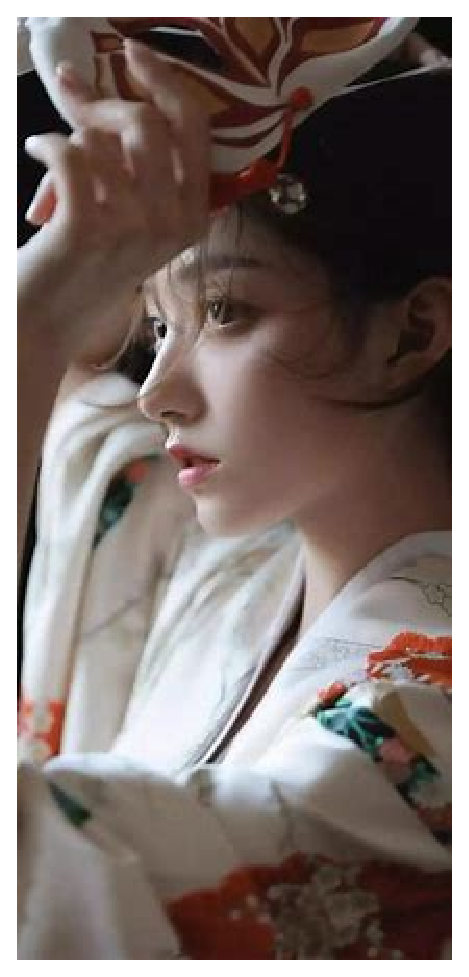
\includegraphics[width=\textwidth]{figures/float_exp_meizi}
        \caption{EPS}
    \end{subfigure}
    \begin{subfigure}[b]{0.32\textwidth}
        
\includegraphics[width=\textwidth]{figures/float_exp_mihoyo}
        \caption{JPG}
    \end{subfigure}
    \caption{网络素材}
    \label{fig:pic}
\end{figure}

\subsection{表格}

长表格一般比较比较难输入,推荐使用工具,如\url{https://tablesgenerator.com/},实在不行用overleaf 自带的也行,长表格如果实在需要断页,一般来说需要标注续表。


\begin{table}[!ht]
\centering % 表格居中
\caption{三线表格} % 表格标题
\label{tab:example} % 用于引用的表格标签
\begin{tabular}{lcr} % lcr表示三列分别左对齐、居中、右对齐
\toprule % 顶部线
\emphasize{左}对齐 & 居中 & \emphasize{右}对齐\\
\midrule % 中间线
$a_1$   & $\int$        &           $\aleph$         \\
$a_1,b_2$   &  $\sum\sum$       &        $ \blacktriangleright \blacktriangleleft$    \\
$a_1,b_2,c_3$    & $\prod\prod\prod$    &   $ \bigstar \circledS  \circlearrowright$   \\
\bottomrule % 底部线
\end{tabular}
\end{table}

\subsection{算法}
算法目前推荐使用\emphasize{algorithm2e}宏包,代码环境一般用
\emphasize{listings}宏包并使用\verb|\lstset|设置风格。

\begin{algorithm}[H]
\DontPrintSemicolon % 不显示分号
\KwData{输入数据}
\KwResult{输出结果}

\SetKwFunction{FMain}{Main}
\SetKwFunction{FSum}{Sum}

\SetKwProg{Fn}{Function}{:}{}
\Fn{\FMain{}}{
  \KwData{这里可以描述函数的输入}
  \KwResult{这里可以描述函数的输出}
  \FSum{$a,b$}\;
  \KwRet{$a+b$}\;
}

\SetKwProg{Fn}{Function}{:}{\KwRet}
\Fn{\FSum{$a, b$}}{
  \KwData{这里可以描述函数的输入}
  \KwResult{这里可以描述函数的输出}
  $sum \gets a + b$\;
  \KwRet{$sum$}\;
}
\caption{示例算法}
\end{algorithm}


\subsection{代码}

\begin{lstlisting}[style=Matlab,caption={MATALB}]
%双曲抛物面
clear;
x = linspace(-10, 10, 100);
y = linspace(-10, 10, 100);
[X, Y] = meshgrid(x, y);
Z = (X.^2)/3 - (Y.^2)/5;
surf(X, Y, Z);  
\end{lstlisting}

\subsection{其他浮动体}
据说支持JavaScript的PDF阅读器,通过\emphasize{media9}宏包,能实现视频或动画的播放。当然利用TikZ(在本文第5节介绍)一帧一帧的放也能实现动画效果,与beamer播放类似。
\clearpage

\section{数学}
\LaTeX 公式符号系统比较完整,不会基本可查,作者虽是数学系但所选数学论文中公式使用的也较少,但还是总结了一些值得注意的坑。
\subsection{数学符号}
\subsubsection{分数}
使用行内公式会显得小,而使用\verb|\dfrac| 会感觉太挤了, 由于行间距一般不能改变,所以要么调行间距,要么使用行间公式,看下面示例
\begin{center}
    \begin{minipage}[c]{4em}
    有志登山顶$\dfrac{3}{9}$, 无志站$\frac{0}{9}$。
\end{minipage}
\end{center}
一般情况分数上下太宽建议直接放在行间。
\subsubsection{积分符号}
一些情况下我们可能需要直立体,而不是斜体。

 牛顿-莱布尼茨公式:
\[ \slantint_a^b f(x)\, dx=F(b)-F(a) , \forall x \in [a,b],F^{\prime}(x)=f(x) \]


高斯定理(散度定理)可以表示为:
\[
\oiint\limits_{\partial V} \mathbf{F} \cdot d\mathbf{S} = \iiint\limits_{V} \nabla \cdot \mathbf{F} \, dV
\]

其中,
\begin{itemize}
    \item $\oiint\limits_{\partial V} \mathbf{F} \cdot d\mathbf{S}$ 表示向量场 $\mathbf{F}$ 通过闭合表面 $\partial V$ 的向外通量,
    \item $\iiint\limits_{V} \nabla \cdot \mathbf{F} \, dV$ 表示向量场 $\mathbf{F}$ 在体积 $V$ 内的散度的积分。
\end{itemize}


\subsubsection{对齐点}
这里align与aligned完全是两个环境,aligned不是一个公式环境,

align:
\begin{align}
 a & = b + c \\
 & = d + e 
 \end{align}
 
 aligned:
 \begin{equation}
 \begin{aligned}
 a&= b+ c\\
 d&= e+ f+g\\
 h+i&= j+k\\
 l+m&= n
 \end{aligned}
 \end{equation}
 对齐需要对齐点,一般在\& 处对齐。
 \subsection{证明、定理和公理}
 本模板序号都用section编号,如果想使用单个序号1,2,3等,当然也可以通过类文件自定义。
 \begin{corollary}
 生活可能不像你想象的那么好,但是也不会像你想象的那么糟,人的脆弱和坚强都超乎了自己的想象,有时候脆弱的一句话会让你泪流满面,有时候你发现自己咬着牙已经走过了很长的路。
 \end{corollary}
 \begin{theorem}[三角形的内积和]
  两直角的平方差一定小于正弦的30°的一半。
 \end{theorem}


\begin{exercise}
子曰:打架用砖乎!不亦乱乎!\hfill ---《论语》
\end{exercise}
\begin{lemma}
 可导函数的每一个可导的极值点都是驻点(函数的导数在该点为零)。
\end{lemma}

\begin{proof}
     利用\[i +j =m\overrightarrow{a}\],可以得到\[\lim_{x+y} =C++\]
\end{proof}
 
\begin{example}[新高考\MakeUppercase{\romannumeral 2}]
想象有$n$个有序排列的箱子,其中每个箱子可以放一个球或者不放球。令二项式系数(或称为组合数) 
$m$ 个球的情况种数。

\end{example}

\begin{solution}
    利用组合数,
    \[ 
      C^m_n= \binom{n}{m} = \frac{n!}{m!(n-m)!}
    \]
    我们可以归纳得出...
\end{solution}


 \clearpage
\newpage
\section{TikZ}
与TikZ有关的\LaTeX 中宏包非常丰富,常规的流程图(附录C图\ref{tikzpicture:process}),函数图,电路图等都有对应的宏包支持,
它的语法也不同于Tex。入门TikZ建议看视频,这一块不建议上来就磕文档,官方文档有上千页。当然其绘图功能也是十分强大!

\begin{figure}[h]
    \centering
    % MergeSort-RecursionTree
% Manuel Kirsch
% \documentclass[a4paper,landscape]{scrartcl}
% %%%<
% \usepackage{verbatim}
% \usepackage[active,tightpage]{preview}
% \PreviewEnvironment{tikzpicture}
% \setlength\PreviewBorder{5pt}%
% %%%>

% % \begin{comment}
% % :Title:  Merge sort recursion tree

% % \end{comment}
% \usepackage{fancybox}
% \usepackage{tikz}

% \title{MergeSort-RecursionTree}
% \author{Manuel Kirsch}
% \date{}
% \begin{document}


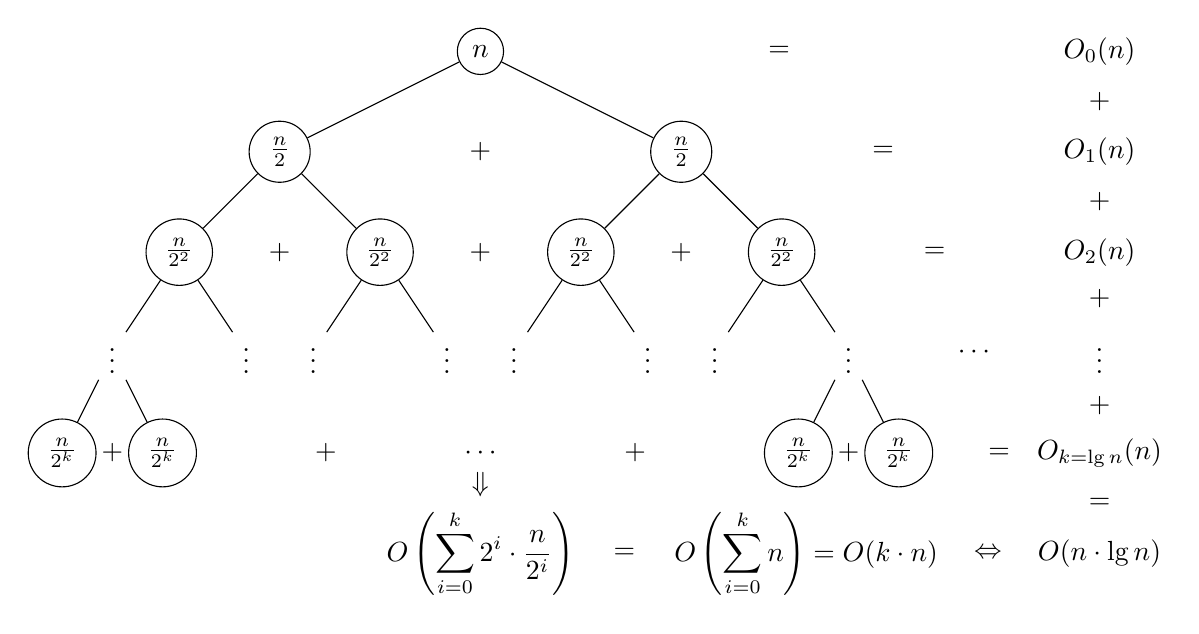
\begin{tikzpicture}[level/.style={sibling distance=60mm/#1},scale=0.85]
\node [circle,draw] (z){$n$}
  child {node [circle,draw] (a) {$\frac{n}{2}$}
    child {node [circle,draw] (b) {$\frac{n}{2^2}$}
      child {node {$\vdots$}
        child {node [circle,draw] (d) {$\frac{n}{2^k}$}}
        child {node [circle,draw] (e) {$\frac{n}{2^k}$}}
      } 
      child {node {$\vdots$}}
    }
    child {node [circle,draw] (g) {$\frac{n}{2^2}$}
      child {node {$\vdots$}}
      child {node {$\vdots$}}
    }
  }
  child {node [circle,draw] (j) {$\frac{n}{2}$}
    child {node [circle,draw] (k) {$\frac{n}{2^2}$}
      child {node {$\vdots$}}
      child {node {$\vdots$}}
    }
  child {node [circle,draw] (l) {$\frac{n}{2^2}$}
    child {node {$\vdots$}}
    child {node (c){$\vdots$}
      child {node [circle,draw] (o) {$\frac{n}{2^k}$}}
      child {node [circle,draw] (p) {$\frac{n}{2^k}$}
        child [grow=right] {node (q) {$=$} edge from parent[draw=none]
          child [grow=right] {node (q) {$O_{k = \lg n}(n)$} edge from parent[draw=none]
            child [grow=up] {node (r) {$\vdots$} edge from parent[draw=none]
              child [grow=up] {node (s) {$O_2(n)$} edge from parent[draw=none]
                child [grow=up] {node (t) {$O_1(n)$} edge from parent[draw=none]
                  child [grow=up] {node (u) {$O_0(n)$} edge from parent[draw=none]}
                }
              }
            }
            child [grow=down] {node (v) {$O(n \cdot \lg n)$}edge from parent[draw=none]}
          }
        }
      }
    }
  }
};
\path (a) -- (j) node [midway] {+};
\path (b) -- (g) node [midway] {+};
\path (k) -- (l) node [midway] {+};
\path (k) -- (g) node [midway] {+};
\path (d) -- (e) node [midway] {+};
\path (o) -- (p) node [midway] {+};
\path (o) -- (e) node (x) [midway] {$\cdots$}
  child [grow=down] {
    node (y) {$O\left(\displaystyle\sum_{i = 0}^k 2^i \cdot \frac{n}{2^i}\right)$}
    edge from parent[draw=none]
  };
\path (q) -- (r) node [midway] {+};
\path (s) -- (r) node [midway] {+};
\path (s) -- (t) node [midway] {+};
\path (s) -- (l) node [midway] {=};
\path (t) -- (u) node [midway] {+};
\path (z) -- (u) node [midway] {=};
\path (j) -- (t) node [midway] {=};
\path (y) -- (x) node [midway] {$\Downarrow$};
\path (v) -- (y)
  node (w) [midway] {$O\left(\displaystyle\sum_{i = 0}^k n\right) = O(k \cdot n)$};
\path (q) -- (v) node [midway] {=};
\path (e) -- (x) node [midway] {+};
\path (o) -- (x) node [midway] {+};
\path (y) -- (w) node [midway] {$=$};
\path (v) -- (w) node [midway] {$\Leftrightarrow$};
\path (r) -- (c) node [midway] {$\cdots$};
\end{tikzpicture}
% \end{document}

    \caption{二叉树}
    \label{tikzpic:tree}
\end{figure}
\begin{figure}[h]
    \centering
     % Pie chart with colors
% Author: Henri Menke
% \documentclass[tikz,border=10pt]{standalone}
% %%%<
% \usepackage{verbatim}
% %%%>
% \begin{comment}
% :Title: Pie chart with colors
% :Tags: Foreach;Charts;Pie charts;Mathematical engine
% :Author: Henri Menke
% :Slug: pie-chart-color

% With this pie chart, we can define a list of colors which is used for the
% pieces. A counter cycles through the list for choosing the color, it restarts
% after the list ended.

% The annotation is done using the pin element.

% This example was written by Henri Menke answering a question of Sascha
% on TeXwelt.de: http://texwelt.de/wissen/fragen/4965/
% \end{comment}
% \begin{document}
\def\angle{0}
\def\radius{3}
\def\cyclelist{{"orange","blue","red","green"}}
\newcount\cyclecount \cyclecount=-1
\newcount\ind \ind=-1


\begin{tikzpicture}[nodes = {font=\sffamily}]
  \foreach \percent/\name in {
      46.6/Chrome,
      24.6/Internet Explorer,
      20.4/Firefox,
      5.1/Safari,
      1.3/Opera,
      2.0/Other
    } {
      \ifx\percent\empty\else               % If \percent is empty, do nothing
        \global\advance\cyclecount by 1     % Advance cyclecount
        \global\advance\ind by 1            % Advance list index
        \ifnum3<\cyclecount                 % If cyclecount is larger than list
          \global\cyclecount=0              %   reset cyclecount and
          \global\ind=0                     %   reset list index
        \fi
        \pgfmathparse{\cyclelist[\the\ind]} % Get color from cycle list
        \edef\color{\pgfmathresult}         %   and store as \color
        % Draw angle and set labels
        \draw[fill={\color!50},draw={\color}] (0,0) -- (\angle:\radius)
          arc (\angle:\angle+\percent*3.6:\radius) -- cycle;
        \node at (\angle+0.5*\percent*3.6:0.7*\radius) {\percent\,\%};
        \node[pin=\angle+0.5*\percent*3.6:\name]
          at (\angle+0.5*\percent*3.6:\radius) {};
        \pgfmathparse{\angle+\percent*3.6}  % Advance angle
        \xdef\angle{\pgfmathresult}         %   and store in \angle
      \fi
    };
\end{tikzpicture}
    

    \caption{扇形图}
    \label{tikzpic:pie}
\end{figure}
\newpage
\begin{figure}[t]
     \centering
     \usetikzlibrary{arrows,shapes,calc,positioning}
\begin{circuitikz}[american]
\draw (0,0) node [scale=1.5,transformer core
] (T){}
      (T.A1) node[above] {A1}
      (T.A2) node[below] {A2}
      (T.B1) node[above left] {B1}
      (T.B2) node[below left] {B2}
      (T.base) node{};
\path (T.B1) -| ++ (2,1) coordinate (tb1){};% define a coordinate at top right relative to B1
\draw (T.B1) -- ++ (0,1) to[D*,-*]  (tb1);
\draw (T.B2) to[D*] ++(2,0)coordinate(tba){} -| (tba |- tb1);
\path (T.B2) |- ++(3,-1) coordinate(tb2){}; % define a coordinate at bottom right relative to B2
\draw (tb2) to[D*,*-] ++(-3,0) -- (T.B2);
\draw (tb2) --(tb2 |- T.B1) to[D*] (T.B1);
% place voltage labels
\draw(T.A1) to[open,v<={$240V_{rms}$,o-o}](T.A2);
\draw($(T.B1)!0.3!(T.B2)$) node[]{$12V_{rms,AC}$}(T.B1);
\draw ($(T.B1)!0.8!(T.B2)$)node[]{$12V_{rms,AC}$}(T.B2);
\draw[thick] ($(T.B1)!0.51!(T.B2)-(1cm,0)$)coordinate[](c){} -- ++ (12.44,0) -| ++ (1,-1) node[ground]{};                          % add a gorund to neutral line
% place capacitors and resistor (upper branches)
\draw(6,1) node[](d1){} to [C,l_=$C_1$, *-*] (c -| d1);
\draw(10,1)node[](d2){} to [C,l_=$C_3$, *-*] (c -| d2);
\draw(13,1)node[](d3){} to [R,l=$R_L$]       (c -| d3);
% place rectangles
\draw (7.5,0.5)  rectangle (8.5,1.5) node[below left= 0.25cm and 0.1cm]{780s};
\draw (7.5,-3.6) rectangle (8.5,-4.6)node[above left=0.25cm and 0.1cm]{790s};
% place capacitors and resistors (lower branches)
\draw(6,-4.15) node[](d4){} to [C,l_=$C_2$, *-*] (c -| d4);
\draw(10,-4.15)node[](d5){} to [C,l_=$C_4$, *-*] (c -| d5);
\draw(13,-4.15)node[](d6){} to [R,l=$R_L$]       (c -| d6);
\draw (8,0.5)  node[](d7){} to [short,-*]        (c -| d7) --(8,-3.6);
% place top and bottom lines
\draw(2,1) -- (7.5,1) (8.5,1) --(11,1) to[short,i^={$I_L$}] (13,1);
\draw(2,-4.15) -- (7.5,-4.15) (8.5,-4.15) --(13,-4.15);
\end{circuitikz}

    \caption{电路图}
    \label{tikzpic:circuit}
\end{figure}

上面的图形都是TikZ代码绘制的,TikZ功能远不止此,由于国内视频缺乏
完整教程,所以学习起来会有些吃力,作者也只是触碰到它的冰山一角,
图\ref{tikzpic:tree} 和图\ref{tikzpic:pie}来自
\url{https://texample.net/tikz},图\ref{tikzpic:circuit}转
载自\href{https://www.latexstudio.net/index/details/index/mid/2302}{latexstudio}。
\section{文献引用与\LaTeX 模板}
\subsection{文献}
本文参考文献的格式为GB/T7714-2015,使用bibtex进行管理,\verb|\cite{}|对文献引用:
\begin{center}

单文件引用\cite{Cheng1999},多个文献引用\cite{CSTAM1990,GBT2659,HBLZ2001,Hopkinson1999,Jiang1989,Jiang1998,Li2000,Li1999,LSC1957,WHO1970,Yu2001,Zhang1998}。
    
\end{center}
\subsection{模板的使用}
想要写出一篇完整论文,除了.cls文件配置的格式文件,写作的过程的其他宏包仍然需要手动添加。本文就是基于xnuthesis.cls编写的,不一定适合所有人,模板提供了一些基础格式,如果需要更精细的格式还需自行重构。
xnuthesis使用的论文组织结构大致如下,更多使用方法可以参考本文的源码,如需学习
撰写类文件可以看\url{https://github.com/rockyzhz/latexdoc-chinese-translation}提供的文档 ,有许多翻译后的中文文档可以参考。

\begin{figure}[p]
\centering
\lstinputlisting[style=LaTex,caption={LaTex论文结构},label={lst:mainstructure}]{main.tex}
\end{figure}

\LaTeXe{}对类文件开发维护困难,主要体现在许多命名规范上的问题 ,于是就产生了\LaTeX 3,\LaTeX 3语法就是由expl3宏包提供的,\url{https://texdoc.org/serve/interface3/0}是\LaTeX 3 语法的完整手册。\LaTeX 3更像是一门面向开发者的编程语言,有类型并且支持函数式编程,命名规范,
缺点是目前还未完全普及,许多宏包还没支持新的l3语法,但这是未来的发展趋势。为了以后兼容性,本模板在类文件中部分也使用了\LaTeX3语法。

\section{总结}
本模板的许多结构方面参考了北航和上交的模板,作者全程依赖GPT解决了许多疑问,不得不说的是
人工智能时代,信息获取方式越来越快,AI已经能实现模块化的基本需求,学习和写出 \LaTeX 程序变得更加轻松了,Typst 与 MathML发展日益强大,也希望某一天能出现更优秀简洁排版方式吧!

\newpage


%========参考文献
\printreferences

%==========致谢
\begin{acknowledgements}
感谢湘南学院提供论文格式!感谢室友及指导老师给出的意见!

\end{acknowledgements}

%========附录
\appendix
{\centering\section{球体}}
这是一个TikZ绘制的3D图形,也是
\href{https://texample.net/tikz/examples/dandelin-spheres/}{example.net/tikz}上面的例子。
\begin{figure}[h]
    \centering
   % Plane Sections of the Cylinder - Dandelin Spheres
% Author: Hugues Vermeiren
% \documentclass{article}
% \usepackage{tikz}
% %%%<
% \usepackage{verbatim}
% \usepackage[active,tightpage]{preview}
% \PreviewEnvironment{tikzpicture}
% \setlength\PreviewBorder{10pt}%
%%%>
% \begin{comment}
% :Title: Plane Sections of the Cylinder - Dandelin Spheres
% :Tags: 3D;mathematical engine;geometry;mathematics
% :Author: Hugues Vermeiren
% :Slug: dandelin-spheres
% \end{comment}
\tikzset{
	MyPersp/.style={scale=1.8,x={(-0.8cm,-0.4cm)},y={(0.8cm,-0.4cm)},
    z={(0cm,1cm)}},
%  MyPersp/.style={scale=1.5,x={(0cm,0cm)},y={(1cm,0cm)},
%    z={(0cm,1cm)}}, % uncomment the two lines to get a lateral view
	MyPoints/.style={fill=white,draw=black,thick}
		}



\begin{tikzpicture}[MyPersp,font=\large]
	% the base circle is the unit circle in plane Oxy
	\def\h{2.5}% Heigth of the ellipse center (on the axis of the cylinder)
	\def\a{35}% angle of the section plane with the horizontal
	\def\aa{35}% angle that defines position of generatrix PA--PB
	\pgfmathparse{\h/tan(\a)}
  \let\b\pgfmathresult
	\pgfmathparse{sqrt(1/cos(\a)/cos(\a)-1)}
  \let\c\pgfmathresult %Center Focus distance of the section ellipse.
	\pgfmathparse{\c/sin(\a)}
  \let\p\pgfmathresult % Position of Dandelin spheres centers
                       % on the Oz axis (\h +/- \p)
	\coordinate (A) at (2,\b,0);
	\coordinate (B) at (-2,\b,0);
	\coordinate (C) at (-2,-1.5,{(1.5+\b)*tan(\a)});
	\coordinate (D) at (2,-1.5,{(1.5+\b)*tan(\a)});
	\coordinate (E) at (2,-1.5,0);
	\coordinate (F) at (-2,-1.5,0);
	\coordinate (CLS) at (0,0,{\h-\p});
	\coordinate (CUS) at (0,0,{\h+\p});
	\coordinate (FA) at (0,{\c*cos(\a)},{-\c*sin(\a)+\h});% Focii
	\coordinate (FB) at (0,{-\c*cos(\a)},{\c*sin(\a)+\h});
	\coordinate (SA) at (0,1,{-tan(\a)+\h}); % Vertices of the
                                           % great axes of the ellipse
	\coordinate (SB) at (0,-1,{tan(\a)+\h});
	\coordinate (PA) at ({sin(\aa},{cos(\aa)},{\h+\p});
	\coordinate (PB) at ({sin(\aa},{cos(\aa)},{\h-\p});
	\coordinate (P) at ({sin(\aa)},{cos(\aa)},{-tan(\a)*cos(\aa)+\h});
     % Point on the ellipse on generatrix PA--PB

	\draw (A)--(B)--(C)--(D)--cycle;
	\draw (D)--(E)--(F)--(C);
	\draw (A)--(E) (B)--(F);
	\draw[blue,very thick] (SA)--(SB);

%	\coordinate (O) at (0,0,0);
%	\draw[->] (O)--(2.5,0,0)node[below left]{x};
%	\draw[->] (O)--(0,3,0)node[right]{y};
%	\draw[->] (O)--(0,0,6)node[left]{z};

	\foreach \t in {20,40,...,360}% generatrices
		\draw[magenta,dashed] ({cos(\t)},{sin(\t)},0)
      --({cos(\t)},{sin(\t)},{2.0*\h});
	\draw[magenta,very thick] (1,0,0) % lower circle
		\foreach \t in {5,10,...,360}
			{--({cos(\t)},{sin(\t)},0)}--cycle;
	\draw[magenta,very thick] (1,0,{2*\h}) % upper circle
		\foreach \t in {10,20,...,360}
			{--({cos(\t)},{sin(\t)},{2*\h})}--cycle;
	\fill[blue!15,draw=blue,very thick,opacity=0.5]
     (0,1,{\h-tan(\a)}) % elliptical section
		\foreach \t in {5,10,...,360}
			{--({sin(\t)},{cos(\t)},{-tan(\a)*cos(\t)+\h})}--cycle;

	\foreach \i in {-1,1}{%Spheres!
		\foreach \t in {0,15,...,165}% meridians
			{\draw[gray] ({cos(\t)},{sin(\t)},\h+\i*\p)
				\foreach \rho in {5,10,...,360}
					{--({cos(\t)*cos(\rho)},{sin(\t)*cos(\rho)},
          {sin(\rho)+\h+\i*\p})}--cycle;
			}
		\foreach \t in {-75,-60,...,75}% parallels
			{\draw[gray] ({cos(\t)},0,{sin(\t)+\h+\i*\p})
				\foreach \rho in {5,10,...,360}
					{--({cos(\t)*cos(\rho)},{cos(\t)*sin(\rho)},
          {sin(\t)+\h+\i*\p})}--cycle;
			}
					\draw[orange,very thick] (1,0,{\h+\i*\p})% Equators
		\foreach \t in {5,10,...,360}
			{--({cos(\t)},{sin(\t)},{\h+\i*\p})}--cycle;
		}
	\draw[red,very thick] (PA)--(PB);
	\draw[red,very thick] (FA)--(P)--(FB);
%	\fill[MyPoints] (CLS) circle (1pt);% center of lower sphere
%	\fill[MyPoints] (CUS) circle (1pt);% center of upper sphere
	\fill[MyPoints] (FA) circle (1pt)node[right]{$F_1$};
	\fill[MyPoints] (FB) circle (1pt)node[left]{$F_2$};
	\fill[MyPoints] (SA) circle (1pt);
	\fill[MyPoints] (SB) circle (1pt);
	\fill[MyPoints] (P) circle (1pt)node[below left]{$P$};
	\fill[MyPoints] (PA) circle (1pt)node[below right]{$P_1$};
	\fill[MyPoints] (PB) circle (1pt)node[above right]{$P_2$};
\end{tikzpicture}


   \caption{dandelin-spheres}
\end{figure}


\newpage
{\centering
\section{说明书}}

C++是一种被广泛使用的计算机程序设计语言。它是一种通用程序设计语言,支持多重编程范式,例如过程化程序设计、面向对象程序设计、泛型程序设计和函数式程序设计等。

比雅尼·斯特劳斯特鲁普博士在贝尔实验室工作期间在20世纪80年代发明并实现了C++。起初,这种语言被称作“C with Classes”(“包含‘类’的C语言”),作为C语言的增强版出现。随后,C++不断增加新特性。虚函数、运算符重载、多继承、标准模板库、异常处理、运行时类型信息、命名空间等概念逐渐纳入标准草案。1998年,国际标准组织颁布了C++程序设计语言的第一个国际标准ISO/IEC 14882:1998,目前最新标准为ISO/IEC 14882:2020。ISO/IEC 14882通称ISO C++。ISO C++包含了主要包含了核心语言和标准库的规则。尽管从核心语言到标准库都有显著不同,ISO C++直接正式(normative)引用了ISO/IEC 9899(通称ISO C),且ISO C++标准库的一部分和ISO C的标准库的API完全相同,另有很小一部分和C标准库略有差异(例如,strcat等函数提供对const类型的重载)。这使得C和C++的标准库实现常常被一并提供,在核心语言规则很大一部分兼容的情况下,进一步确保用户通常较容易把符合ISO C的源程序不经修改或经极少修改直接作为C++源程序使用,也是C++语言继C语言之后流行的一个重要原因。

作为广泛被使用的工业语言,C++存在多个流行的成熟实现:GCC、基于LLVM的Clang以及Visual C++等。这些实现同时也是成熟的C语言实现,但对C语言的支持程度不一(例如,VC++对ANSI C89之后的标准支持较不完善)。大多数流行的实现包含了编译器和C++部分标准库的实现。编译器直接提供核心语言规则的实现,而库提供ISO C++标准库的实现。这些实现中,库可能同时包含和ISO C标准库的共享实现(如VC++的msvcrt);而另一些实现的ISO C标准库则是单独于编译器项目之外提供的,如glibc和musl。C++标准库的实现也可能支持多种编译器,如GCC的libstdc++库支持GCC的g++和LLVM Clang的clang++。这些不同的丰富组合使市面上的C++环境具有许多细节上的实现差异,因而遵循ISO C++这样的权威标准对维持可移植性显得更加重要。现今讨论的C++语言,除非另行指明,通常均指ISO C++规则定义的C++语言(虽然因为实现的差异,可能不一定是最新的正式版本)。




\newpage
{\centering
\section{流程图}}
\begin{figure}[h]
    \centering
   % Diagram of Android activity life cycle
% Author: Pavel Seda 
% \documentclass[border=10pt]{standalone}
% %%%<
% \usepackage{verbatim}
% %%%>
% \begin{comment}
% :Title: Diagram of Android activity life cycle
% :Tags: Diagrams;Flowcharts;Charts;Styles;Computer science
% :Author: Pavel Seda
% :Slug: android

% A flow diagram of an Android activity life cycle.
% It uses basic nodes and arrows and defines node styles.
% \end{comment}
% \usepackage{tikz}
% \usetikzlibrary{arrows.meta}
\tikzset{%
  >={Latex[width=2mm,length=2mm]},
  % Specifications for style of nodes:
            base/.style = {rectangle, rounded corners, draw=black,
                           minimum width=4cm, minimum height=1cm,
                           text centered, font=\sffamily},
  activityStarts/.style = {base, fill=blue!30},
       startstop/.style = {base, fill=red!30},
    activityRuns/.style = {base, fill=green!30},
         process/.style = {base, minimum width=2.5cm, fill=orange!15,
                           font=\ttfamily},
}
% \begin{document}    
% Drawing part, node distance is 1.5 cm and every node
% is prefilled with white background
\begin{tikzpicture}[node distance=1.5cm,
    every node/.style={fill=white, font=\sffamily}, align=center]
  % Specification of nodes (position, etc.)
  \node (start)             [activityStarts]              {Activity starts};
  \node (onCreateBlock)     [process, below of=start]          {onCreate()};
  \node (onStartBlock)      [process, below of=onCreateBlock]   {onStart()};
  \node (onResumeBlock)     [process, below of=onStartBlock]   {onResume()};
  \node (activityRuns)      [activityRuns, below of=onResumeBlock]
                                                      {Activity is running};
  \node (onPauseBlock)      [process, below of=activityRuns, yshift=-1cm]
                                                                {onPause()};
  \node (onStopBlock)       [process, below of=onPauseBlock, yshift=-1cm]
                                                                 {onStop()};
  \node (onDestroyBlock)    [process, below of=onStopBlock, yshift=-1cm] 
                                                              {onDestroy()};
  \node (onRestartBlock)    [process, right of=onStartBlock, xshift=4cm]
                                                              {onRestart()};
  \node (ActivityEnds)      [startstop, left of=activityRuns, xshift=-4cm]
                                                        {Process is killed};
  \node (ActivityDestroyed) [startstop, below of=onDestroyBlock]
                                                    {Activity is shut down};     
  % Specification of lines between nodes specified above
  % with aditional nodes for description 
  \draw[->]             (start) -- (onCreateBlock);
  \draw[->]     (onCreateBlock) -- (onStartBlock);
  \draw[->]      (onStartBlock) -- (onResumeBlock);
  \draw[->]     (onResumeBlock) -- (activityRuns);
  \draw[->]      (activityRuns) -- node[text width=4cm]
                                   {Another activity comes in
                                    front of the activity} (onPauseBlock);
  \draw[->]      (onPauseBlock) -- node {The activity is no longer visible}
                                   (onStopBlock);
  \draw[->]       (onStopBlock) -- node {The activity is shut down by
                                   user or system} (onDestroyBlock);
  \draw[->]    (onRestartBlock) -- (onStartBlock);
  \draw[->]       (onStopBlock) -| node[yshift=1.25cm, text width=3cm]
                                   {The activity comes to the foreground}
                                   (onRestartBlock);
  \draw[->]    (onDestroyBlock) -- (ActivityDestroyed);
  \draw[->]      (onPauseBlock) -| node(priorityXMemory)
                                   {higher priority $\rightarrow$ more memory}
                                   (ActivityEnds);
  \draw           (onStopBlock) -| (priorityXMemory);
  \draw[->]     (ActivityEnds)  |- node [yshift=-2cm, text width=3.1cm]
                                    {User navigates back to the activity}
                                    (onCreateBlock);
  \draw[->] (onPauseBlock.east) -- ++(2.6,0) -- ++(0,2) -- ++(0,2) --                
     node[xshift=1.2cm,yshift=-1.5cm, text width=2.5cm]
     {The activity comes to the foreground}(onResumeBlock.east);
  \end{tikzpicture}
% \end{document}

    \caption{android}
    \label{tikzpicture:process}
\end{figure}

\end{document}
